%! TEX root = thesis.tex

\chapter{Theoretical Concepts}%
\label{sec:fundamentals}

Till now, we have understood the problem statement we want to tackle and the applications. We also understood that it takes knowledge about multiple domains to bridge the gap towards songs to lyrics transcription. In this chapter, we will build on the introduction and give a detailed background about the Acoustic Modelling techniques that will be utilized for Feature Extraction, Automatic Speech Recognition(ASR) systems that will give a blueprint for modelling Songs to Lyrics Transcription and performing transfer learning from the Speech to the Songs domain, and Music Information Retrieval (MIR) domain that will help us to isolate Singing Voice from the instruments to be utilized within the proposed songs to lyrics transcription system. The proposed system will be covered in Chapter 3 but this chapter will give the required prerequisites that will be needed to understand the proposed system.

\section{Acoustic Modelling}%
\label{sec:acousticmodelling}

The Acoustic Modelling section will talk about Feature Extraction methodologies that are typically used within the Audio domain. We will be employing some of the following techniques within our proposed system.

\subsection{Spectrograms}%
\label{sec:spectrograms}

Spectrograms are visual representations of frequencies of an audio signal across time scale. In the spectrogram representation, the horizontal axis represents time and the vertical axis represents the frequencies. The color represents the amplitude of the observed frequencies at a particular point of time. To illustrate, the following image in Figure \ref{fig:spectrogram} shows a spectrogram that has been created from an audio file  \cite{mcfee2015librosa}  . The presence of bright colors at certain places show the amplitude of the frequency at those times in the audio wave.

\begin{figure}
     \centering
     \begin{subfigure}[b]{0.48\textwidth}
         \centering
         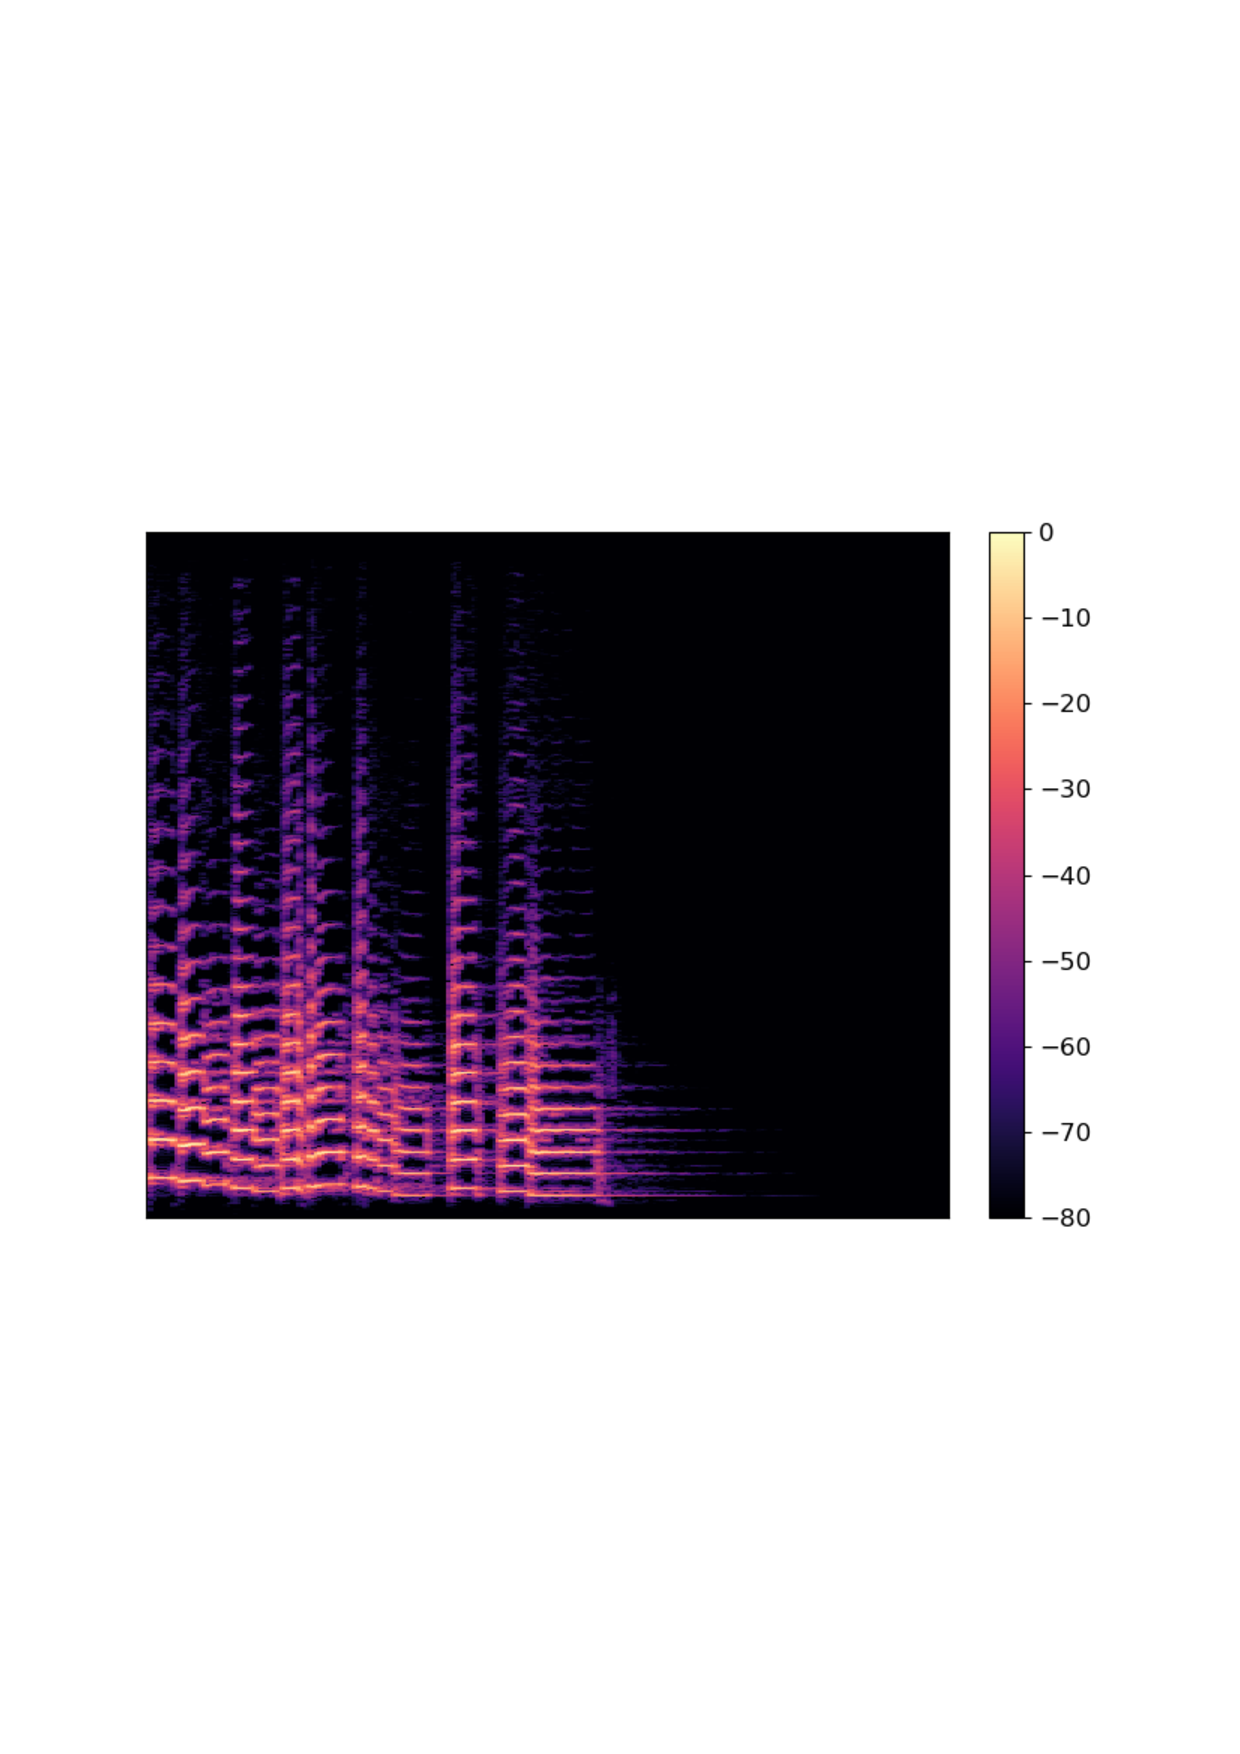
\includegraphics[width=\textwidth]{03-Theoretical Foundations/figures/spectrogram.pdf}
         \caption{Spectrogram}
         \label{fig:spectrogram}
     \end{subfigure}
     \hfill
     \begin{subfigure}[b]{0.48\textwidth}
         \centering
         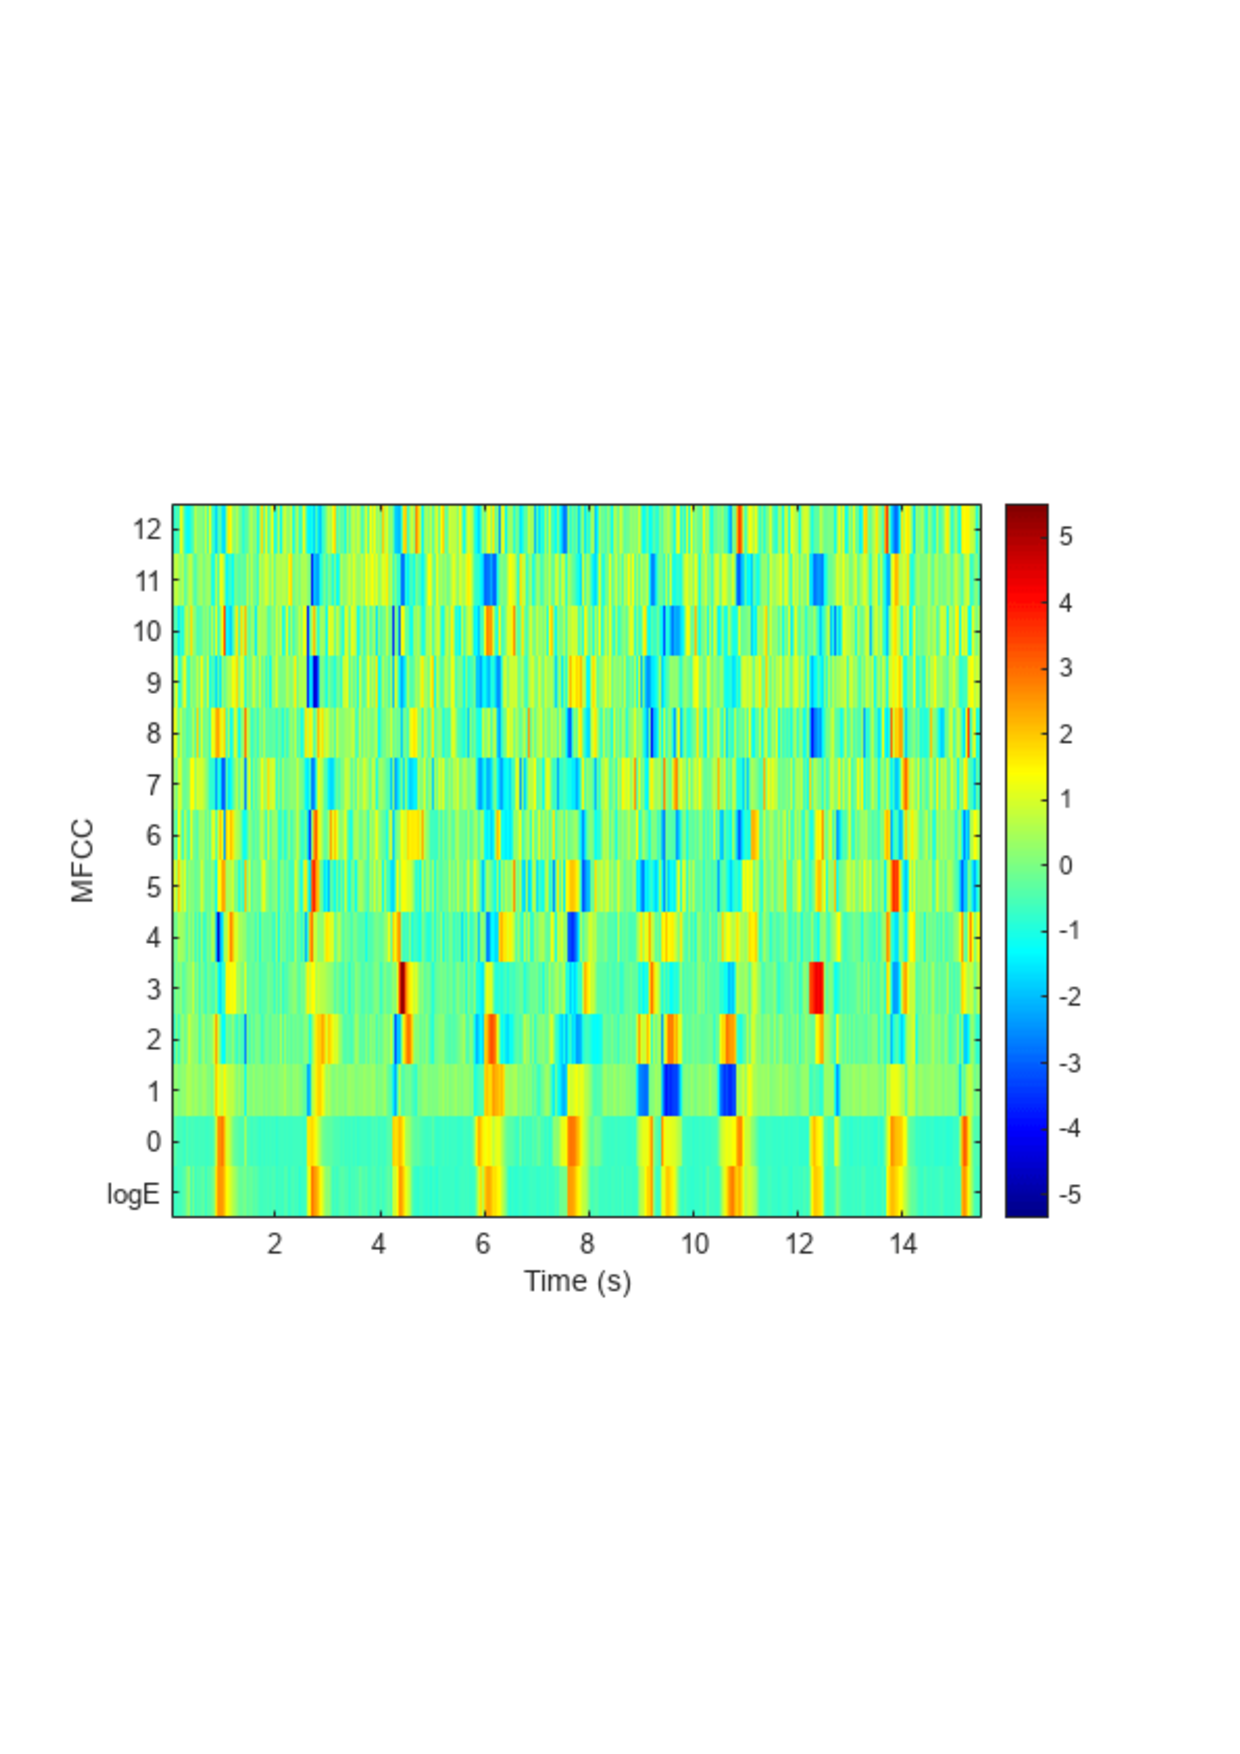
\includegraphics[width=\textwidth]{03-Theoretical Foundations/figures/mfcc_matlab.pdf}
         \caption{Mel Frequency Cepstral Coefficients}
         \label{fig:mfcc}
     \end{subfigure}
     \hfill
        \caption{Acoustic Feature Extraction Techniques}
        \label{fig:acoustic_feature_extract}
\end{figure}

In order to create the spectrogram, the audio signal is broken down into smaller frames or windows. Following this, Discrete Fourier Transform (or Fast Fourier Transform) is used on each window to get the frequencies for each window within the time frame of that audio wave. It is also a common practice to keep overlapping windows so that we don't lose the frequencies. In the Songs to lyrics transcription domain, we will be interested in taking windows of 20ms to 30ms as it is roughly the minimum time for a phoneme to be spoken by humans. This way, we will be able to capture all the phonemes being sung by the singer. Also, typical overlap between two frames is kept at 50\% (typically it is between 25\% and 75\%). Once the Fourier of the windows have been calculated, the absolute values of the complex valued amplitudes are calculated and normalized. The resultant matrix is plotted and the spectrogram is obtained.

By plotting the spectrograms, we can convert the problem from an audio to text (multimodal) classification problem to a Multiclass Image Classification problem to perform lyrics transcription. We will be using the librosa \cite{mcfee2015librosa} python package for plotting the spectrograms. In modern architectures such as Whisper, which we will look into later in this chapter, we will see how variants of Spectrograms will be fed into deep learning models to automatically learn a function of the spectrogram to the transcription, allowing for a general approximation of the problem.

\subsection{Mel Frequency Cepstral Coefficients (MFCC)}%
\label{sec:mfcc}

A special variant of the spectrograms is Mel Frequency Cepstral Coefficients (MFCC). This lossless audio feature extraction methodology, as plotted in \ref{fig:mfcc}, is a technique that creates 39 features that emulate the vocal pattern of the human throat and the hearing pattern of the ear. To illustrate, a human being hears frequencies from 20Hz to 20kHz. Within that spectrum, a tune of 300 Hz will be as similar as the sound of a standard dial tone of a landline telephone. In comparison, a 400 Hz will sound slightly higher. However, the human mind will practically interpret the distance between the two frequencies as negligible and somewhat the same. However, when the human ear listens to a 900Hz audio signal, a 1KHz sound appears distinctly different. The Mel-frequency Cepstral coefficients (MFCCs)  feature extraction is created on similar lines and leverages logarithms to capture the contrast of the differences as shown through the following formula:

\begin{equation}
{Mel}(f)=2595 \log \left(1+\frac{f}{700}\right)
\end{equation}

Since an audio signals keeps changing in its characteristics, we create 20ms -40ms frames of the signal as seen in the previous section \ref{sec:spectrograms} and assume that the audio signal is statistically stationary within the frame. This helps us to create Mel-frequency Cepstral coefficients (MFCCs) in an iteraive fashion throughout the entire length of the audio signal. As seen in the Figure \ref{fig:mfccgeneration}, the steps to generate the Mel-frequency Cepstral coefficients (MFCCs)  are outlined below \cite{huang2001spoken} \cite{song2016detecting}:
\begin{itemize}
    \item Window the audio signal into small frames.
    \item For each overlapping frame, calculate the periodogram estimate of power spectrum \cite{song2016detecting}
    \item Apply Mel Filterbank to the power spectra on the above mentioned features and then sum the energy in the filters.
    \item Calculate the logarithm of all Filterbank energies.
    \item Calculate the discrete cosine transform of the obtained values.
    \item From the previous step, keep features s 2-13, discard the rest.
\end{itemize}


\begin{figure}
    \centering
    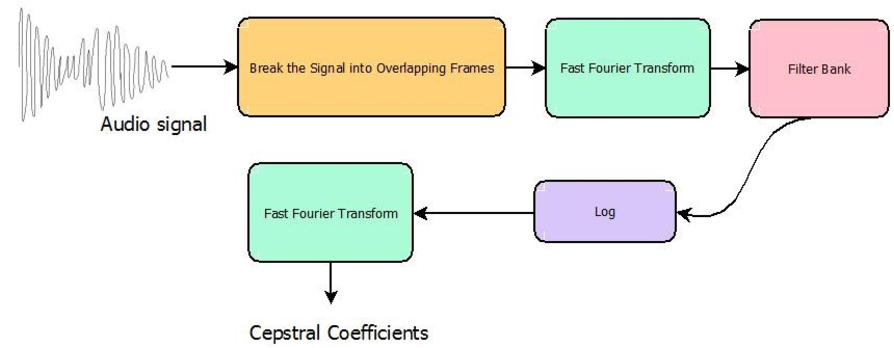
\includegraphics[width=1.0\textwidth]{03-Theoretical Foundations/figures/mfcc_generation.pdf}
    \caption{Process to generate MFCC}
    \label{fig:mfccgeneration}
\end{figure}


The 39 Features generated through the above mechanisms are an input to the Automatic Speech Recognition (ASR) system. In our Songs to Lyrics Transcription problem, we will be using the MFCC features for performing transfer learning in the Whisper model in order to adapt the domain from the speech to the songs domain.


\subsection{Hidden Markov Models(HMM)}%
\label{sec:hmm}

The Hidden Markov Models(HMM) is a variant of the Markov Chain model. To give a background, the Markov Chain is a model that provides probabilities of sequences of random states and how it transitions from one state to another \cite{gales2008application}. The Markov Chain model, and in extension, Hidden Markov Models (HMM) assume finite number of states and a stationary distribution for transitioning from one state to another. A key defining element of the Markov family of models are that the current state is all that matters to predict the future. The states prior to the current state have zero impact on the future.

To understand this mathematically, let us consider a sequence of state variables $q_1,q_2,...,q_i$. The Markov assumption can be represented as follows :

\begin{equation}
P(q_i = a|q_i...q_{i-1})\ =\ P(q_i=\ a|q_{i-1})
\end{equation}

While Markov Chains are used to calculate the probability for a sequence of observable events, it doesn't provide a probability distribution over hidden events. For example, identifying the phoneme associated with an acoustic features in an acoustic signal cannot be done through Markov Chains. Here is where Hidden Markov Models (HMM) shine. Assume $Q = q_1, q_2 ... q_N$ represents the state of the Hidden Markov Model (HMM),  $A_{ij}$ being the transition probability matrix, where $\sum_{j\ =\ 1}^{N}{a_{ij}\ =\ 1}$   $\forall{i}$, and $O = ,o_1,o_2, ...o_T$ are the observation likelihoods that emanate from the hidden states $Q$, then the Hidden Markov Model assumption looks like the one below:

\begin{equation}
P\left(o_i \mid q_1 \ldots q_i, \ldots, q_T, o_1, \ldots, o_i, \ldots, o_T\right)=P\left(o_i \mid q_i\right)
\end{equation}

To train a Hidden Markov Models(HMM) for calculating the likelihoods of observations for an acoustic model, algorithms that can be leveraged are the Forward-Backward Algorithms, Baum-Welch Algorithm or Expectation-Maximization Algorithm. One mechanism to overcome the limitation of the model to be dependent only on the current state is to have N gram models. In this way, we can model a state as a history of N events. This gives us the ability to add history but the cost is an explosion in the number of states within the model. Once we have a trained Hidden Markov Models(HMM), Inference can be performed using Viterbi or the Forward-Backward Algorithm.

\section{Automatic Speech Recognition(ASR)}%
\label{sec:e2easrsystems}

\begin{figure} [H]
    \centering
    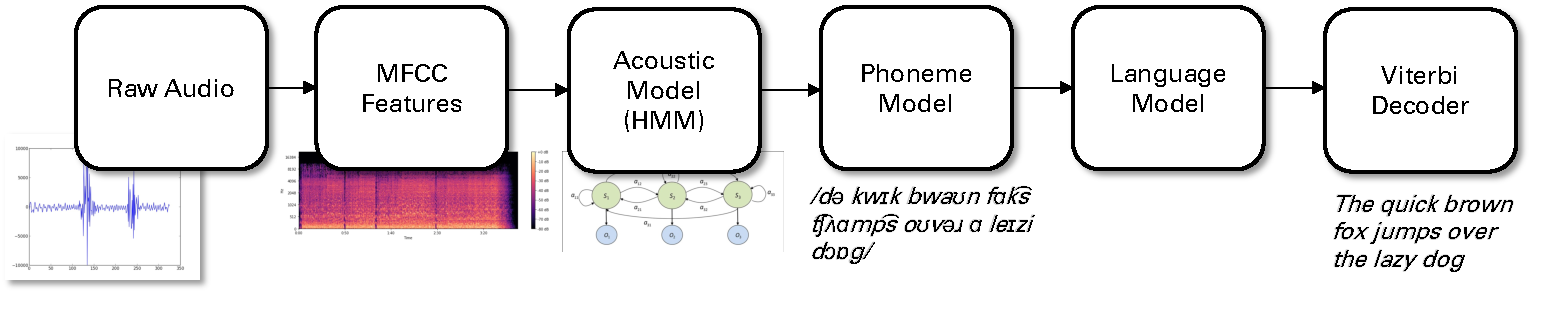
\includegraphics[width=0.9\textwidth]{03-Theoretical Foundations/figures/e2e_asr.pdf}
    \caption{End to End Automatic Speech Recognition Systems}
    \label{fig:e2easr}
\end{figure}

Automatic Speech Recognition is a field that takes speech audio as an input and outputs the transcription of the speech. The traditional automatic speech recognition (ASR) system has several stages as part of the end to end model as shown in figure \ref{fig:e2easr}. The raw audio inputs are fed into feature extractor that converts it into Mel Frequency Cepstral Coefficients (MFCC). Post that, an acoustic model is trained that takes these 39 features as inputs and outputs the phonemes. Acoustic Models have traditionally been done by leveraging Hidden Markov Models (HMM). This is then decoded into phoneme using Phoneme model that provides the probability of seeing a letter when seeing a phoneme $P(letter_i/Phoneme_i)$ and the language model that provides the probability of the next word given the current word $P(word_i/word_{i-1})$. Finally, the decoding is done by using Viterbi Algorithm.

\begin{figure} [H]
    \centering
    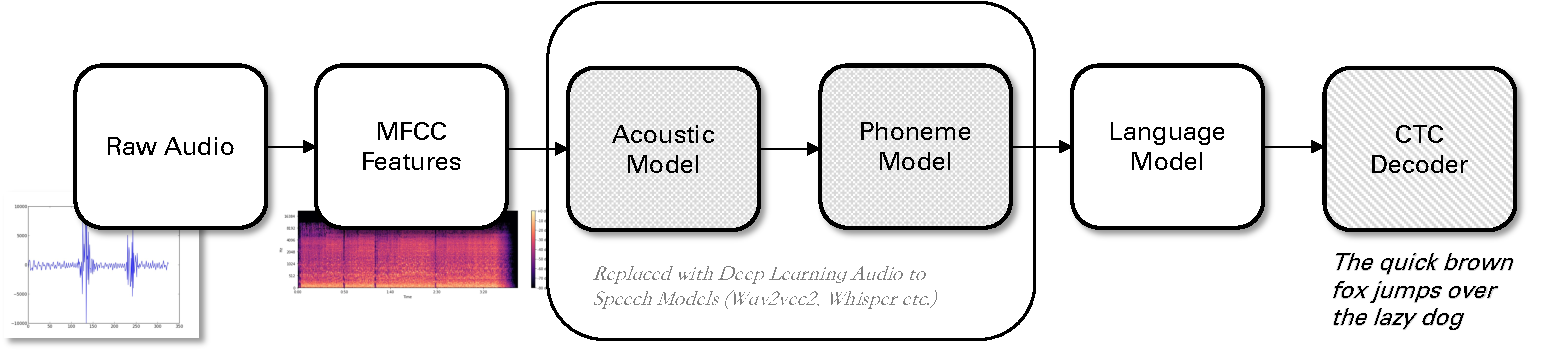
\includegraphics[width=0.9\textwidth]{03-Theoretical Foundations/figures/deeplearning_asr_systems.pdf}
    \caption{End to End Automatic Speech Recognition Systems}
    \label{fig:deepasr}
\end{figure}


In modern contexts, there are no separate acoustic model and a phoneme model. Deep Learning architectures such as Wav2Vec2 are able to output transcription (text) from the models. Another model Whisper, which we will see in this section, also includes a decoder and the language model included within the architecture through an encoder-decoder architecture. This helps to greatly simplify the architecture.


\subsection{Wav2Vec2.0 Model Architecture}%
\label{sec:wav2vec2}



\begin{figure} [H]
    \centering
    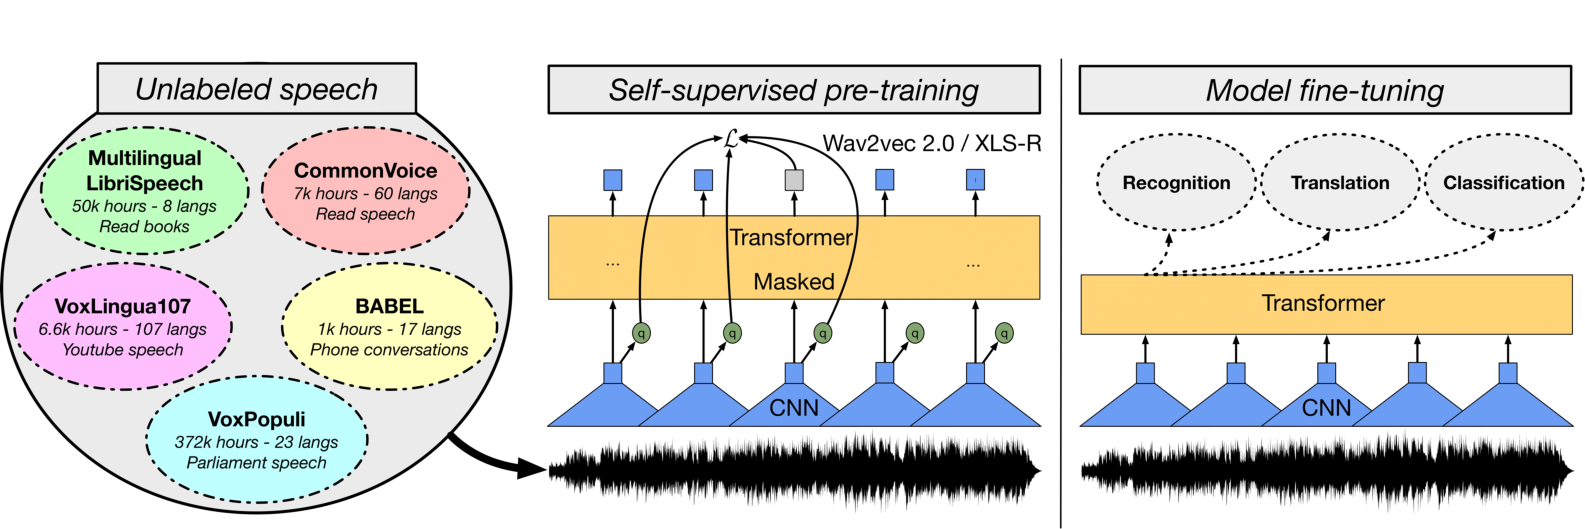
\includegraphics[width=1.0\textwidth]{03-Theoretical Foundations/figures/wav2vec2 asr.pdf}
    \caption{Wav2Vec2: A Framework for Self-Supervised
Learning of Speech Representations}
    \label{fig:wav2vec2}
\end{figure}


Wav2Vec2.0 is a framework that consists of two stages - (1) the pre-training step which leverages self-supervised learning techniques that will be briefly outlined below and (2) A fine-tuning step where a language model head is added on top of the pre-trained model to perform speech recognition, translation etc. The pre-training process is self-supervised and hence doesn't require labelled data. The training of the model in this step uses a contrastive loss and helps to differentiate audio features from each other. In the fine-tuning step, the audio features are obtained from the pre-trained model and using language heads, outputs a pre-trained model that can learnt  self-supervised learning of representations from raw audio data. Basically it learns to efficiently represent the raw audio data as a vector space encoding. A major advantage of this approach is that we end up training a generic audio model that can be used to differentiate the different sounds and create features for them, while the downstream tasks can be specialized for tasks such as Speech Recognition, Translation or Classification. Another benefit of this approach is that there is an ample amount of unlabelled audio data while only a fraction of the data has actual high quality labels associated with them. In the paper, after pre-training on unlabeled speech, the model is fine-tuned on smaller labeled data with a Connectionist Temporal Classification (CTC) loss for speech recognition task.

The complete architecture of the framework can be divided into 3 components, they are

\textbf{Feature encoder}: This part represents the encoder part and takes audio signals as input and provides feature vectors as outputs. The input size is typically 400 samples of 20ms for 16KHz sampled audio. The features are extracted by first standardizing the input to have zero mean and unit variance, followed by a 1-D Convolution neural network and a layer normalization with GELU activation function. There are typically 7 such convolution blocks with an output vector size of 512 dimensions.

\textbf{Transformers}: The output from the first section is passed into the Transformer layer that learns to differentiate between the different features extracted for the different samples. In Wav2Vec2, the original transformer architecture is slightly modified by leveraging relative positional embedding instead of fixed positional encoding. The block size is 12 transformers with an output of 768 dimensions in the Base model and 1024 dimensions in the Large model.

\textbf{Quantization module}: The quantization module converts the continuous speech input into discrete units, so that it is compatible with self-supervised learning. To do so, this module maintains multiple code-books or groups (320 in size) and sampling is done from these code-books using Gumbel Soft-max, which is a differentiable variant of the \texttt{argmax}).

The training objective for the pre-training step is to minimize the contrastive loss and diversity loss. Contrastive loss, as mentioned earlier, is to differentiate between the audio units while having the diversity loss helps the algorithm from making use of the entire quantized code-book. For the Songs Lyrics Transcription (SLT) space, we will be using a classification layer on top of the transformer layer with a size equal to the vocabulary size and a goal of minimizing the Connectionist temporal classification(CTC) Loss. Pre-training was done with an Adam optimizer.
To make the model more robust to different tasks, we can fine-tune the model on a different task specific modifications and dataset. Here, the paper fine-tuned for ASR by adding a randomly initialized classification layer on top on Transformer layer with class size equal to the size of vocab. The model's objective is optimized by minimizing the Connectionist temporal classification(CTC) loss with the Adam Optimizer. The learning rate is warmed up for 10\% of the duration of training, then kept constant for 40\% and then linear decayed for the remainder of the training. For the first 60,000 updates, the output classifier was trained and only post that was the Transformer is also updated. The feature encoder is kept frozen.

\subsection{Whisper - Weak Supervised Learning for Speech Recognition}%
\label{sec:whisper}

\begin{figure} [H]
    \centering
    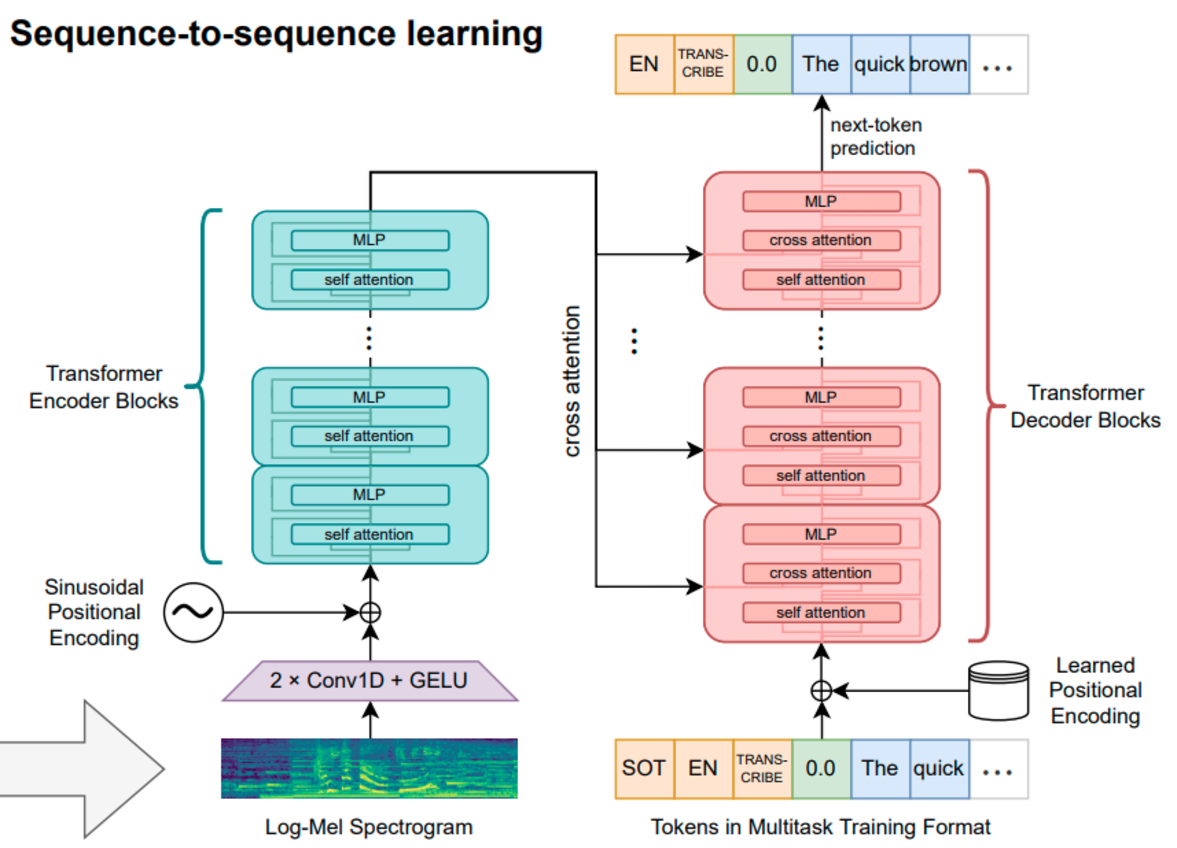
\includegraphics[width=0.9\textwidth]{03-Theoretical Foundations/figures/whisper.pdf}
    \caption{Whisper Model Architecture}
    \label{fig:whisper}
\end{figure}


The Whisper model is an encoder-decoder architectural model that solves the Automatic Speech Recognition problem in an end to end fashion. In this model, input audio is first split into 30 second chunks and then converted into Mel Frequency Cepstral Coefficients (MFCC) features as we saw in section \ref{sec:mfcc}. Then, the features are passed to the transformer architecture based encoder. The output of this is the encoder hidden states that is passed to the decoder that auto-regressively predicts the next token given the encoder hidden state as context and the previous tokens available. For this type of architecture to work, there is a need for a large amount of labelled audio data. To make this work, the whisper architecture was trained on 0.68 million hours of weakly labelled data, the largest such dataset ever created. The model is the state of the art model that performs competitively on a wide variety of tasks and long form transcription in comparison to Wav2vec2 architectures. When Whisper's zero shot performance is tracked across diverse datasets, it produces 50\% fewer errors than the Wav2vec2 models. However, on domains (datasets) that were part of the Wav2vec2 training, , the Wav2vec2 model outperforms on these benchmarks.

\section{Music Information Retrieval (MIR)}%
\label{sec:musicinformationretrieval}

Music information retrieval (MIR) is the domain related to music and information that explores the retrieval of information from science.

\begin{itemize}
    \item Music generation
    \item Music Genre classification
    \item Music Recommender systems
    \item Singing Voice Separation
    \item Automatic music transcription

\end{itemize}

Within this domain, we are, in particular, interested in the Music Source Separation problem. This subdomain within the Music Information Retrieval (MIR) domain aims to extract the vocal components from music. The motivation for doing so is to reduce the noise that we will have from accompanied instruments for the songs to lyrics transcription problem statement.

\subsection{Music Source Separation using Hybrid DEMUCS}%
\label{sec:demucs}

\begin{figure} [H]
    \centering
    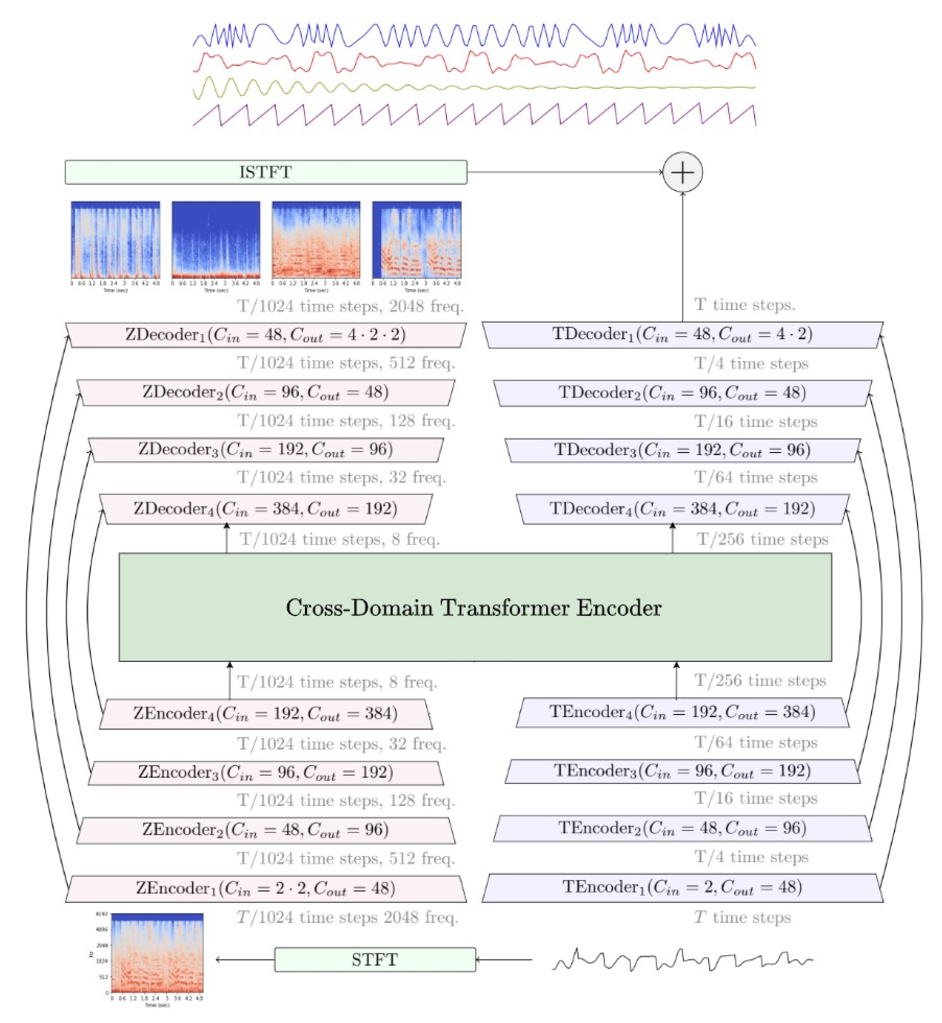
\includegraphics[width=0.9\textwidth]{03-Theoretical Foundations/figures/demucs.pdf}
    \caption{Music Source Separation using DEMUCS}
    \label{fig:demucs}
\end{figure}


In order to extract the lyrics from the songs, the essential component of the songs needed is the vocal tracks as it contains the lyrics completely in audio form. Hence, as part of a pre-processing step, it is interesting to look at extracting the singing voice alone from the songs. To do this, there are different algorithms that have been developed such as Spleeter \cite{spleeter2020} and DEMUCS \cite{rouard2022hybrid} that are the current state of the arts. Spleeter leverages Deezer internal datasets and a U-net architecture, that is an encoder-decoder Convolutional Neural Network (CNN) architecture with skip connections. The training was done using a L1-norm loss between masked input mix spectrograms and source target spectrograms. Hybrid DEMUCS also leverages a similar architecture and is based on the U-Net like network architecture that extracts waveform patterns. Since, it is convolution based, it leverages Mel Spectrograms as image inputs. As shown in figure \ref{fig:demucs}, it is an encoder-decoder architecture with bi-directional LSTMs to take into account temporal dimensions of the inputs. On the output side, it is a stereo estimate for each sound source. The entire solution is trained on MUSDB dataset with an additional 800 songs and is the state of the art benchmark for the MUSDB dataset.



\section{Decoding Procedures}%
\label{sec:decoders}

Automatic Speech Recognition (ASR) Models typically output logits from a classification layer(soft-max) that is of the size of the vocabulary of the model. This is true also for both ASR models outlined in this thesis - the Wav2vec2 with language head (classification layer) and Whisper. In order to represent them and convert them into lyrics, we can employ different methodologies to do so. The following points detail a quick summary of the techniques in this space. We will go into the Songs Lyrics Transcription part of it when we see it as part of the experimentation in the next chapter. \\

The different decoding techniques are as follows:

\begin{itemize}
    \item \textbf{Greedy Decoding \cite{zhang2023dive}} : In this methodology, the \textit{argmax} of the logits are taken and the most probable item in the vocabulary makes it as lyrics in a concatenated fashion.
    \item \textbf{CTC Decoding with Greedy \cite{sutskever2014sequence}}: This is similar to the above method but in addition, it avoids duplicate letters from coming to the final lyrics and corrects them through CTC algorithm.
    \item \textbf{Beam Search \cite{zhang2023dive}} : Beam Search is a breadth first heuristic search algorithm that explores a graph of promising possibilities in a limited fashion. For example, if a beam of 3 is selected, it will explore the graph of 3 possibilities in every step of the prediction and finally selecting the most probable lyrics from all possibilities. While this helps boost accuracy, it increases the memory complexity and decreases the speed of decoding for the model.
    \item  \textbf{Beam Search with Language Models \cite{sutskever2014sequence}}: In this methodology, in addition to beam search, a language model is created that understands the domain of lyrics and basically provides an additional probability the sentence within the beam, allowing for more accurate lyrics to be generated.
\end{itemize}

\section{Discussion}%
\label{sec:foundationaltheorydiscussion}

In this particular chapter, we have seen in detail the different components that we will be interested in to develop the Songs to Lyrics Transcription System and where they might add value within the songs to lyrics transcription proposed system. We have given our motivations for exploring these domains as they will be used in our experiments and research to transcribe songs to lyrics. In the next chapter, we will see the problem formulation, evaluation methodology, hardware and software setup that we have employed for our thesis. In addition, we will outline the research questions and hypothesis we have defined in order to improve the benchmarks in the songs to lyrics transcription problem.
